\documentclass[]{article}
\usepackage{multirow}
\usepackage{amsmath}
\usepackage{circuitikz}
\usepackage{graphicx}
\usepackage[italian]{babel}
\usepackage{float}
\textwidth=450pt\oddsidemargin=0pt
\usepackage{geometry}
\geometry{a4paper, top=2cm, bottom=2cm, left=2cm, right=2cm,  heightrounded, bindingoffset=5mm}
%opening
\title{Misura della caratteristica I-V di due diodi a giunzione p-n}
\author{Cristina Caprioglio, Luca Morelli}
\date{Primo turno, tavolo 3}

\begin{document}

\maketitle

\section{Scopo della prova}
La prova consisteva nella misura delle caratteristiche I-V di due diodi a giunzione p-n, uno al Silicio e uno al Germanio. Abbiamo realizzato una serie di fit con ROOT in modo da ricavare i parametri caratteristici del diodo: la corrente inversa ``$  I_{0}$" e ``$\eta V_{T}$", il prodotto tra il fattore di idealità e l'equivalente della temperatura in volt. 
\section{Procedura}
	\begin{figure}[H]
		\centering
		\begin{circuitikz}
			\draw
			(0,4) node[above]{$Ground$} to[short, *-]
			(0,2) to[potentiometer, -, l=1$ k\Omega $] (2,2) 
			(2.5,0) node[below]{$B$} to[empty diode, *-*] (1.25,0)node[below]{$A$}--(0,0)--(0,2)
			(2,4) node[above]{$+5V$} to[short, *-] (2,2)
			;
			\draw [<-]
			(1,1.5)--(1,1)--(2,1);
			\draw
			(2,1)--(2.5,1) node[above]{$C$} to[short, *-] (3,1)
			to[short, -*] (3, 3.5)node[above]{$(Rosso)$} (3.5, 4)node[above]{$Multimetro$}
			;
			\draw
			(4,3.5)node[above]{$(Nero)$} to[short, *-] (4,0)--(3.5,0)node[below]{$D$}to[short, *-](2.5,0)
			;
		\end{circuitikz}
	\label{fig:schema}
	\caption{Schema del circuito realizzato}
	\end{figure}


Per prima cosa abbiamo eseguito la calibrazione della tensione misurata con l'oscilloscopio, mettendola in relazione con quella data dal multimetro. Per fare ciò abbiamo collegato l'oscilloscopio al punto C (figura 1) e abbiamo cortocircuitato i punti A-B per poi procedere a prendere 10 misure tra i 50 e i 760 mV. Per ogni misura abbiamo prima preso il valore dell'oscilloscopio e poi quello del multimetro.\\
Spostando poi il potenziometro fuori dal circuito ne abbiamo regolato la resistenza a $ 500 \,\Omega $, per poi reinserirlo nella sua posizione iniziale. Abbiamo quindi inserito il diodo tra i punti A e B (figura 1), prima quello al Silicio e poi quello al Germanio, entrambi con il catodo nel punto A. Dopo aver spostato il probe dell'oscilloscopio nel punto D abbiamo effettuato 16 misure per il Silicio e 23 per il Germanio, agendo sul potenziometro per variare la tensione e leggendo poi la corrente dal multimetro. \\Infine, abbiamo fittato i dati raccolti per ottenere i parametri ricercati.
\section{Materiali utilizzati}
\begin{itemize}
	\item Potenziometro da $ 1 \,k\Omega $
	\item Diodo p-n: AAZ15/OA47 Germanio
	\item Diodo p-n: 1N914A/1N4446/1N4148 Silicio
	\item Cavetti
	\item Cacciavite
	\item Cavi a doppia banana
	\item Breadboard
\end{itemize}
\section{Strumentazione}
\begin{itemize}
	\item Alimentatore a bassa tensione
	\item Oscilloscopio ISO-TECH, ISR 622 20MHz
	\item Multimetro digitale ISO-TECH, IDM 105
\end{itemize}
\section{Misurazioni}
La tabella (1) di seguito riporta i valori relativi a fondo scala, risoluzione e precisione dei vari strumenti:
	\begin{table}[H]
		\centering
		\begin{tabular}{|c|c|c|c|}
			\cline{2-4}
			\multicolumn{1}{c|}{} & Fondo scala & Risoluzione & Precisione \\
			\hline
			\multirow{4}{*}{Oscilloscopio (mV)} & 10 & 2 & 3\% \\
			\cline{2-4}
			& 50 & 10 & 3\% \\
			\cline{2-4}
			& 100 & 20 & 3\% \\
			\cline{2-4}
			& 200 & 40 & 3\% \\
			\hline
			\multirow{2}{*}{Multimetro (mV)} & 400 & 0.1 & 0.3\%$+2d$ \\
			\cline{2-4}
			&$4\cdot10^3$ & 1 & 0.1\%$+2d$\\
			\hline
			Multimetro (mA) & 4 - 400 & $10^{-3}$ & 0.4\%$+2d$ \\
			\hline
		\end{tabular}
	\label{tab:strumenti}
	\caption{Dati forniti dai data sheet della strumentazione utilizzata}
	\end{table}
Per il calcolo degli errori relativi alle misure effettuate con l'oscilloscopio si è usata la seguente formula:
\begin{equation}
	\sigma=\sqrt{(\sigma_{L})^{2}+(\sigma_{Z})^{2}+(\sigma_{C})^{2}}
\end{equation}
dove $\sigma_{C}= (misura\cdot0.03) $ è l'errore del costruttore. 
\begin{equation*}
	\sigma_{L}=\sigma_{Z}=\frac{fondo \:scala}{5}\cdot\#tacchette \:apprezzabili
\end{equation*}
$ \sigma_{Z} $ è l'errore sullo zero, in tal caso il fondo scala vale 10 mV/div.\\
Invece $ \sigma_{L} $ è l'errore sulla lettura e in questo caso il fondo scala varia in base alla misura, mentre ``\#tacchette apprezzabili" é stato considerato 0.5 per tutte le misure.
Per gli errori relativi al multimetro abbiamo preso la misura e moltiplicata rispettivamente per 0.3\% , 0.1\% o 0.4\%  in base al fondo scala usato, poi abbiamo arrotondato all'ordine di grandezza della risoluzione ed aggiunto due digit.
\subsection{Calibrazione dell'oscilloscopio}
La tabella a seguire (\ref{tab:calibrazione}) riporta le misure utilizzate per calibrare l'oscilloscopio: per ogni misura è riportato il fondo scala utilizzato poichè, come si può vedere in tabella (1), questo influenza la stima dell'errore. 
	\begin{table}[H]
		\centering
	\begin{tabular}{|c|c|c|c|}
		\hline
		Tensione oscilloscopio (mV)& Fondo scala oscillos. (mV/div) & Tensione multimetro (mV) & Fondo scala mult. (mV) \\
		\hline
		$ 50\pm 2 $ &$ 10 $ & $ 48.2\pm 0.3 $ &400\\
		\hline
		$ 130\pm 6$ &$ 50 $ & $ 123.4\pm 0.6 $ &400\\
		\hline
		$ 210\pm 8 $ &$ 50 $ & $ 202.6\pm 0.8 $ &400\\
		\hline
		$ 280\pm 10$ &$ 100 $ & $ 269\pm 1 $ &400\\
		\hline
		$ 360\pm 20 $ &$ 100 $ & $ 349\pm 1 $ &400\\
		\hline
		$ 440\pm 20 $ &$ 100 $ & $ 428\pm 2 $ &4$\cdot10^3$\\
		\hline
		$ 520\pm 20 $ &$ 100 $ & $ 505\pm 3 $ &4$\cdot10^3$\\
		\hline
		$ 600\pm 30 $ &$ 200 $ & $ 571\pm 3 $ &4$\cdot10^3$\\
		\hline
		$ 680\pm 30 $ &$ 200 $ & $ 654\pm 3 $&4$\cdot10^3$ \\
		\hline
		$ 760\pm 30 $ &$ 200 $ & $ 734\pm 3 $&4$\cdot10^3$ \\
		\hline
		
	\end{tabular}
\caption{Punti sperimentali della calibrazione dell'oscilloscopio}
\label{tab:calibrazione}
\end{table}
\subsection{Silicio}
Nella seguente tabella (\ref{tab:silicio}) sono riportati i punti sperimentali acquisiti per la caratteristica I-V del diodo al Silicio, per ogni misura è riportato il fondo scala utilizzato poichè, come si può vedere in tabella (1), questo influenza la stima dell'errore.

	\begin{table}[H]
		\centering
	\begin{tabular}{|c|c|c|c|}
		\hline
		Tensione oscilloscopio (mV)& Fondo scala (mV/div) & Corrente multimetro (mA) &Fondo scala (mA)\\
		\hline
		$ 420\pm 20 $ &$ 100 $ & $ 0.016\pm 0.002 $ &4\\
		\hline
		$440\pm20 $ &$ 100 $ & $ 0.025\pm0.002 $ &4 \\
		\hline
		$ 460\pm 20 $ &$ 100 $ & $ 0.038\pm 0.002 $ &4 \\
		\hline
		$ 500\pm 20 $ &$ 100 $ & $ 0.082\pm 0.002 $ &4 \\
		\hline
		$ 520\pm 20 $ &$ 100 $ & $0.121\pm 0.002$ &4 \\
		\hline
		$ 540\pm 20 $ &$ 100 $ & $ 0.185\pm 0.003 $ &4 \\
		\hline
		$ 550\pm 20 $ &$ 100 $ & $ 0.213\pm 0.003 $ &4 \\
		\hline
		$ 560\pm 20 $ &$ 100 $ & $ 0.284\pm 0.003 $ &4 \\
		\hline
		$ 570\pm 20 $ &$ 100 $ & $ 0.297\pm 0.003 $ &4 \\
		\hline
		$ 580\pm 20 $ &$ 100 $ & $ 0.350\pm 0.004 $ &4 \\
		\hline
		$ 600\pm 30 $ &$ 200 $ & $ 0.602\pm0.004 $  &4\\
		\hline
		$ 620\pm 30 $ &$ 200 $ & $ 0.738\pm0.005 $  &4\\
		\hline
		$ 640\pm 30 $ &$ 200 $ & $ 1.207\pm0.007 $  &4\\
		\hline
		$ 680\pm 30 $ &$ 200 $ & $ 2.24\pm 0.01 $ &4 \\
		\hline
		$ 720\pm 30 $ &$ 200 $ & $ 2.62\pm 0.01 $ &4 \\
		\hline
		$ 760\pm 30 $ &$ 200 $ & $ 3.70\pm 0.02 $ &4 \\
		\hline
			\end{tabular}
		\caption{Punti acquisiti per la caratteristica I-V del Silicio}
		\label{tab:silicio}
	\end{table}
\subsection{Germanio}
Nella tabella (\ref{tab:germanio}), sotto riportata, sono presentati i punti sperimentali acquisiti per la caratteristica I-V del diodo al Germanio, per ogni misura è riportato il fondo scala utilizzato poichè, come si può vedere in tabella (1), questo influenza la stima dell'errore.
	\begin{table}[H]
		\centering
	\begin{tabular}{|c|c|c|c|}
		\hline
		Tensione oscilloscopio (mV)& Fondo scala (mV/div) & Corrente multimetro (mA) &Fondo scala (mA)\\
		\hline
		$ 70\pm 6 $ &$ 50 $ & $ 0.014\pm 0.002 $ &4 \\
		\hline
		$ 80\pm 6$ &$ 50 $ & $ 0.020\pm 0.002 $&4 \\
		\hline
		$ 90\pm 6$ &$ 50 $ & $ 0.026\pm 0.002 $&4 \\
		\hline
		$ 100\pm 6 $ &$ 50 $ & $ 0.034\pm 0.002 $&4 \\
		\hline
		$110\pm 6 $ &$ 50 $ & $ 0.045\pm 0.002 $&4 \\
		\hline
		$ 120\pm 6 $ &$ 50 $ & $ 0.056\pm 0.002 $&4 \\
		\hline
		$ 130\pm 6$ &$ 50 $ & $ 0.071\pm 0.002 $&4 \\
		\hline
		$ 140\pm 7$ &$ 50 $ & $ 0.089\pm 0.002 $&4 \\
		\hline
		$ 150\pm 7$ &$ 50 $ & $ 0.109\pm 0.002 $&4 \\
		\hline
		$ 160\pm 7$ &$ 50 $ & $ 0.134\pm 0.003 $&4 \\
		\hline
		$ 170\pm 7$ &$ 50 $ & $ 0.162\pm 0.003 $&4 \\
		\hline
		$ 180\pm 7$ &$ 50 $ & $ 0.200\pm 0.003 $&4 \\
		\hline
		$ 190\pm 8$ &$ 50 $ & $ 0.244\pm 0.003 $&4 \\
		\hline
		$ 200\pm 8$ &$ 50 $ & $ 0.305\pm 0.003 $&4 \\
		\hline
		$ 210\pm 8$ &$ 50 $ & $ 0.323\pm 0.003 $&4 \\
		\hline
		$ 220\pm 8$ &$ 50 $ & $ 0.441\pm 0.004 $&4 \\
		\hline
		$ 230\pm 9$ &$ 50 $ & $ 0.451\pm 0.004 $&4 \\
		\hline
		$ 240\pm 9$ &$ 50 $ & $ 0.537\pm 0.004 $&4 \\
		\hline
		$ 250\pm 9$ &$ 50 $ & $ 0.712\pm 0.005 $&4 \\
		\hline
		$ 260\pm 9$ &$ 50 $ & $ 0.730\pm 0.005 $&4 \\
		\hline
		$ 270\pm 10$ &$ 50 $ & $ 0.850\pm 0.005 $&4 \\
		\hline
		$ 280\pm 10$ &$ 50 $ & $ 0.990\pm 0.006 $&4 \\
		\hline
		$ 290\pm 10$ &$ 50 $ & $ 1.118\pm 0.006 $&4 \\
		\hline
	\end{tabular}
\caption{Punti acquisiti per la caratteristica I-V del Germanio}
\label{tab:germanio}
\end{table}
\section{Elaborazione dati e risultati}

La prima fase di elaborazione dati consiste nella verifica della calibrazione dell'oscilloscopio, questa ci ha premesso di valutare la miglior stima dell'errore su quest'ultimo. In seguito abbiamo proseguito fittando i dati sperimentali delle tabelle (formula \ref{tab:silicio}) e (formula \ref{tab:germanio}) per ottenere i parametri caratteristici dei diodi con relativi errori, ottenuti tramite somma in quadratura per tenendo conto della presenza di dati non indipendenti tra loro. Per ogni diodo abbiamo effettuato due fit: uno esponenziale (figura \ref{fitexp}) e uno lineare (figura \ref{fitlin}) pesato utilizzando i logaritmi delle correnti misurate.
\begin{equation}
	I(V)=I_0(e^{\frac{V}{\eta V_T}}-1)
	\label{fitexp}
\end{equation}
\begin{equation}
	Y=a+bX \quad con\quad Y=V,\: X=lnI, \:a=-\eta V_{T}lnI_{0},\: b=\eta V_{T}%Siamo sicuri sia giusta?
	\label{fitlin}
\end{equation}
Infine abbiamo riportato i risultati su appositi grafici assieme ai punti sperimentali in modo da costruire graficamente la curva I-V. 
  \subsection{Calibrazione dell'oscilloscopio}
Il fit dei dati in tabella (\ref{tab:calibrazione}), riportato nel grafico in figura \ref{fig:calibrazione}, ha evidenziato un chiaro comportamento lineare con pendenza $1.03662\pm0.0004$ e intercetta pari a $(0.4\pm0.4)mV$.
\begin{figure}[H]
	\centering
	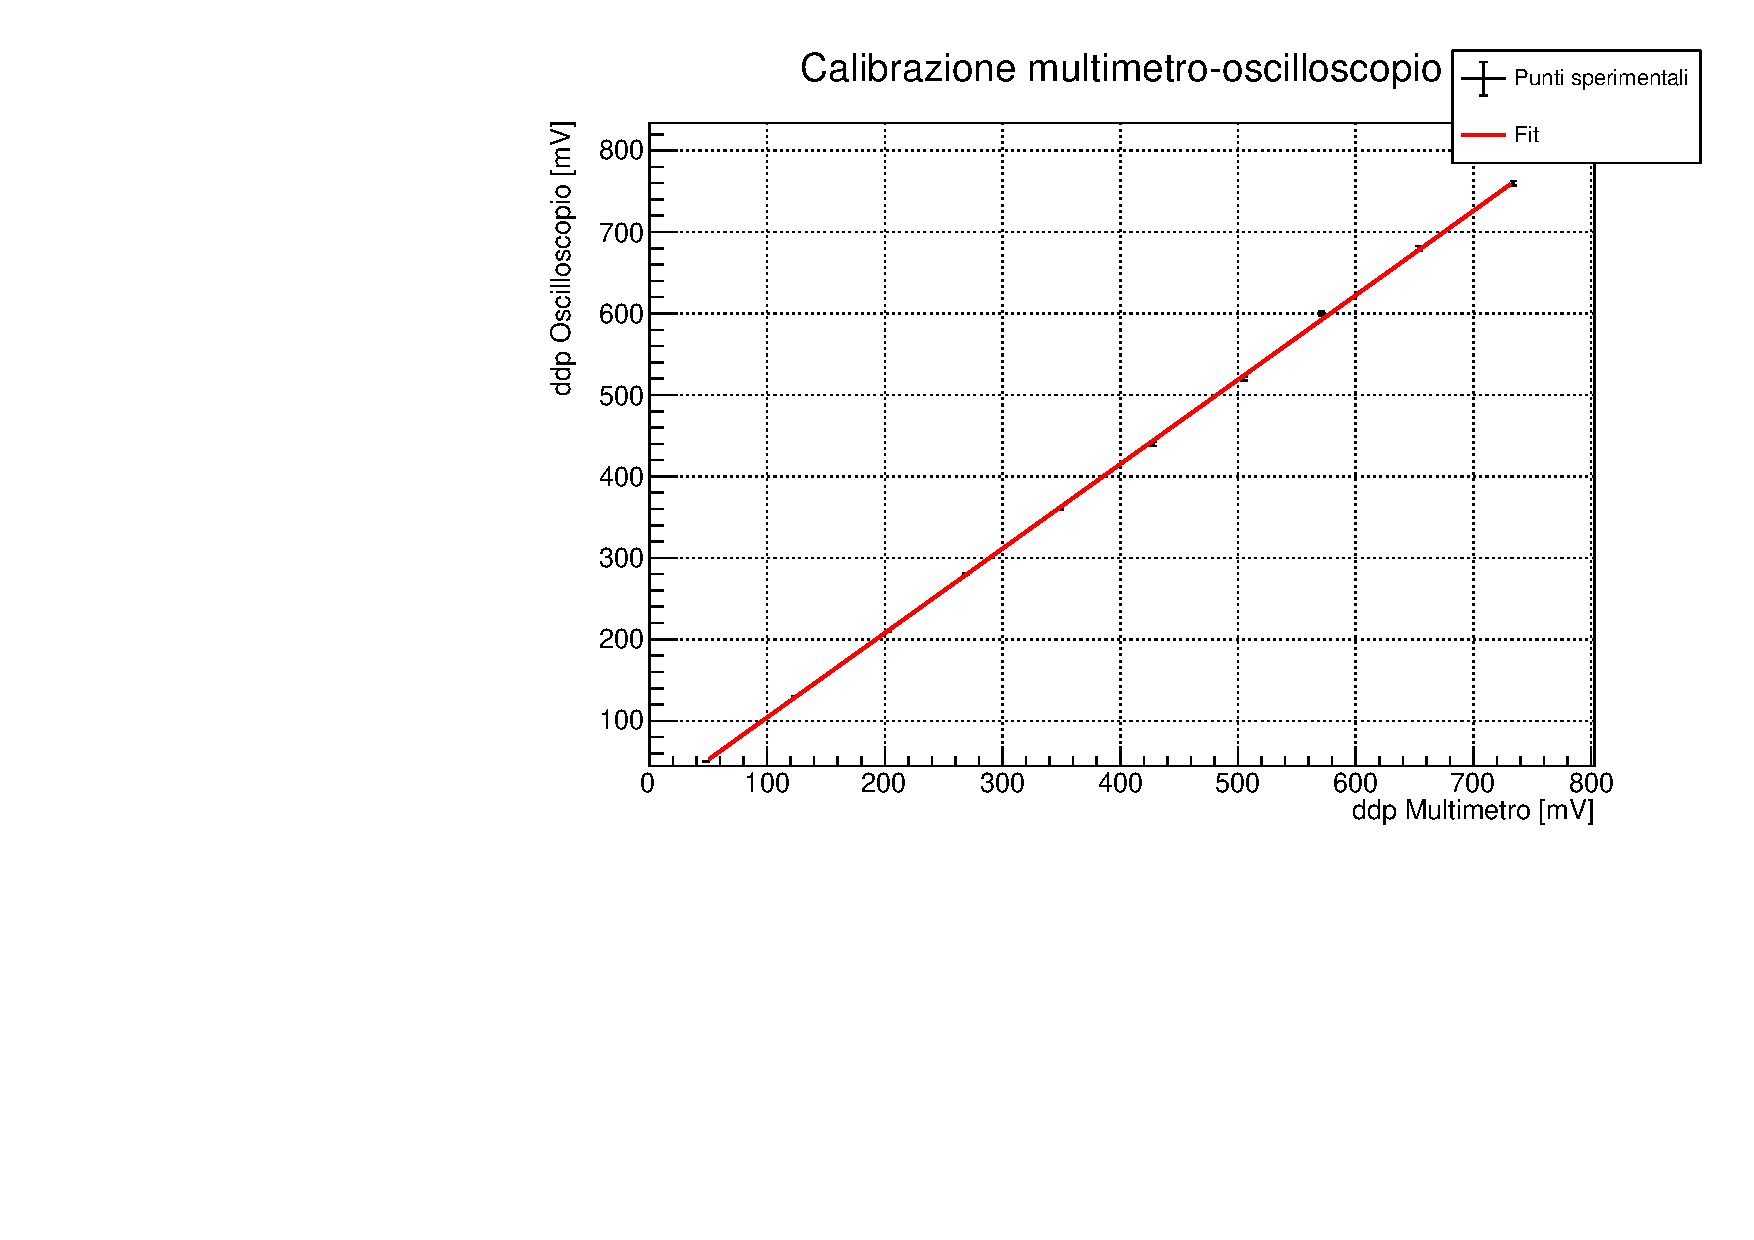
\includegraphics[width=0.4\linewidth]{../Silicio/Calibrazione}
	\caption{Retta di calibrazione delle tensioni dell'oscilloscopio}
	\label{fig:calibrazione}
\end{figure}
Questa misura ci ha permesso di considerare trascurabili eventuali errori dovuti alla calibrazione dello strumento poichè questi risultano chiaramente inferiori agli errori strumentali da noi valutati e riportati nelle tabelle (\ref{tab:silicio}) e (\ref{tab:germanio}).
\subsection{Silicio}
Dai dati in tabella (\ref{tab:silicio}), come già spiegato, abbiamo effettuato due fit, riportati graficamente in figura (\ref{fig:silicio}): quello esponenziale ci ha concesso di stimare $I_0=(5\pm5)nA$ e $\eta V_T=(51\pm5)mV$, mentre quello lineare ha restituito valori di $I_0=(7.2\pm0.7)nA$ e $\eta V_T=(53\pm4)mV$. Per entrambi i fit non abbiamo utilizzato tutti i punti sperimentali raccolti, ma abbiamo valutato quale fosse il range di fit migliore alla luce del fatto che dopo un certo valore di soglia il comportamento caratteristico muta dalla legge ideale, come è possibile apprezzare negli ultimi punti rappresentati, seppur non utilizzati, del grafico semilogaritimico in figura(\ref{fig:silicio}). 
Per il fit esponenziale abbiamo utilizzato il range $[400mV-650mV]$ mentre per il fit lineare il range $[400mV-600mV]$.
\begin{figure}[H]
	\centering
	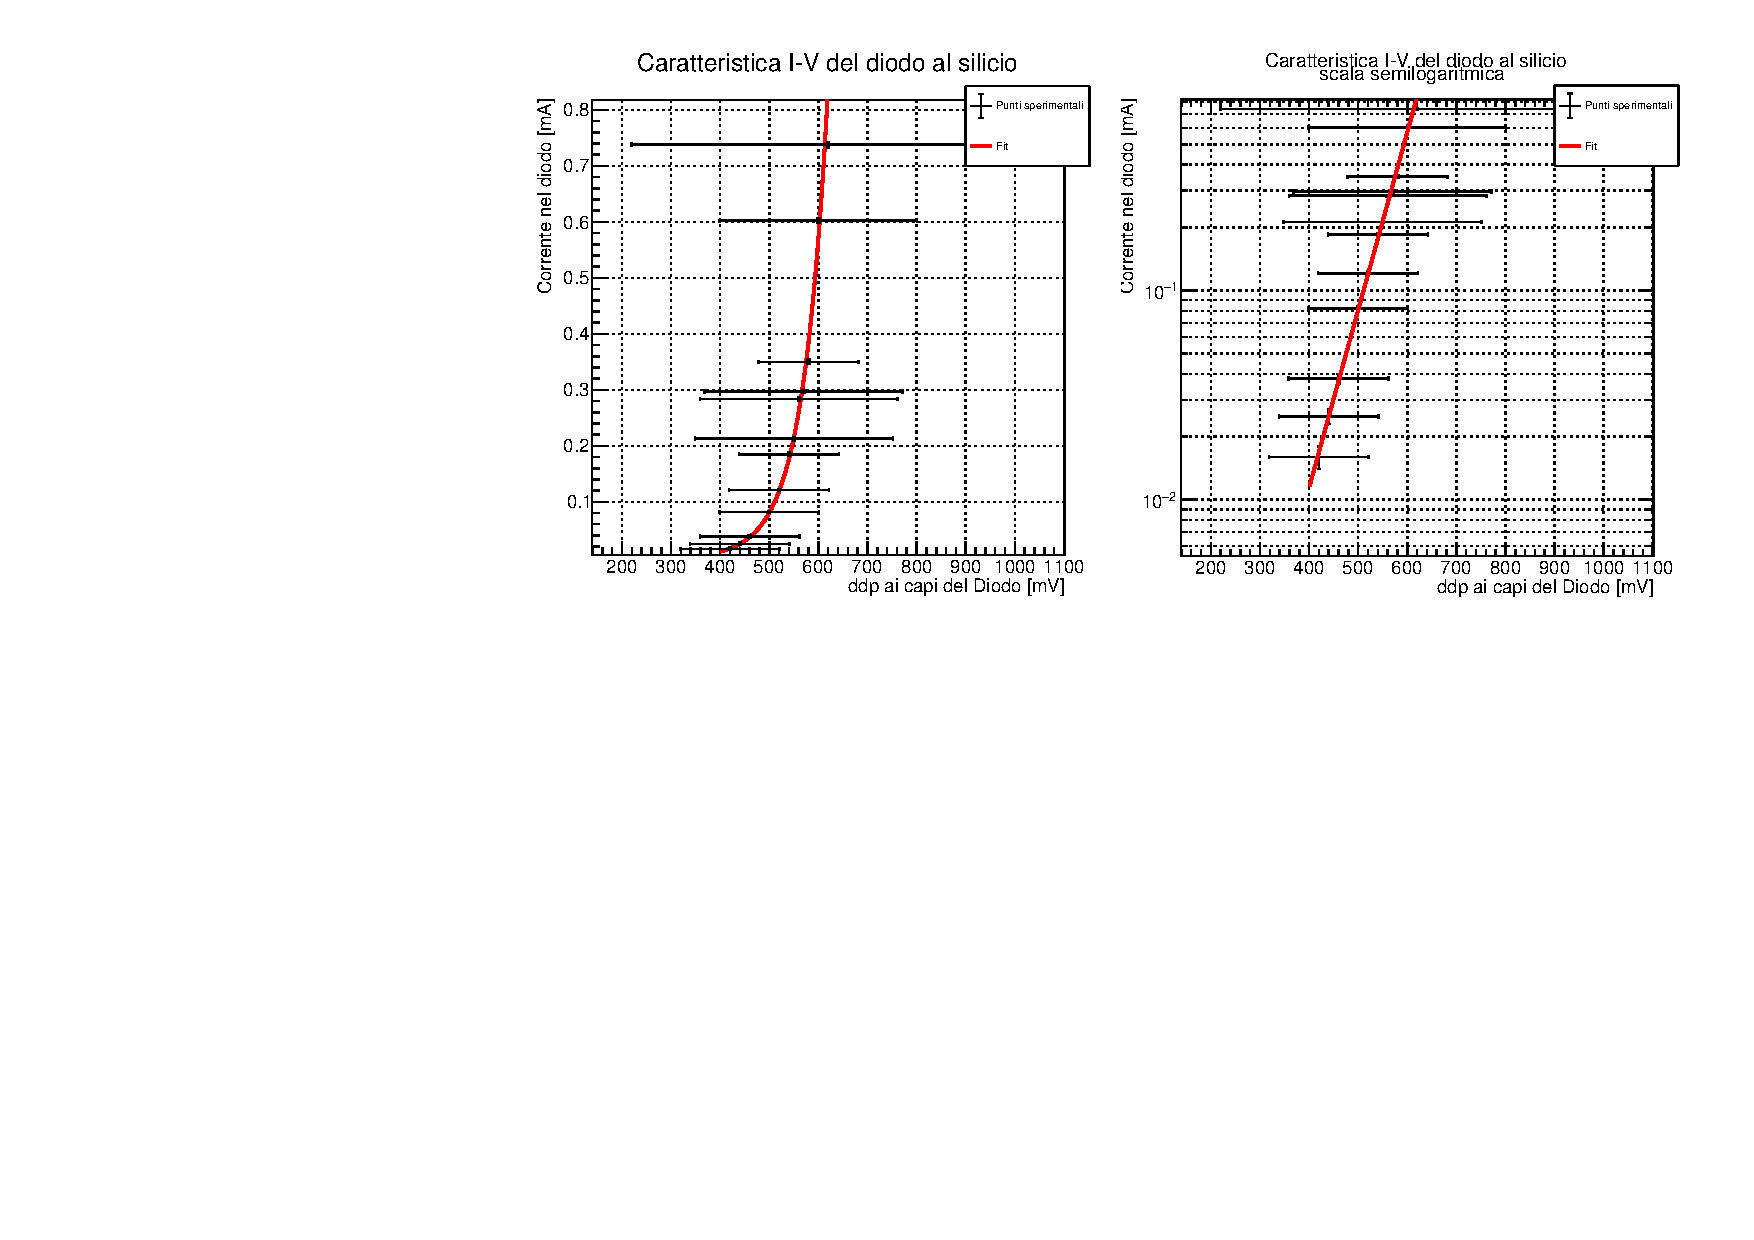
\includegraphics[width=0.8\linewidth]{../Silicio/canvas}
	\caption{Caratteristica I-V del diodo al Silicio: a sinistra sono riportati i punti nel range utilizzato per effettuare il fit esponenziale mentre a destra sono riportati tutti i punti sperimentali in scala semilogaritmica con fit lineare}
	\label{fig:silicio}
\end{figure}
Osserviamo che le misure ottenute dai due fit sono compatibili tra loro seppur il fit lineare si riveli più preciso riuscendo a stimare con un errore minore il parametro $I_0$.
I parametri misurati si rivelano in questo caso in accordo con quelli attesi.
\subsection{Germanio}
I fit effettuati e riportati graficamente in figura (\ref{fig:germanio}) hanno concesso di stimare $I_0=(4\pm1)\mu A$ e $\eta V_T=(43\pm5)mV$ (fit esponenziale) e $I_0=(2.6\pm0.3)\mu A$ e $\eta V_T=(40\pm3)mV$ (fit lineare). Anche in questo caso per entrambi i fit non abbiamo usato tutti i punti sperimentali raccolti. La deviazione dal comportamento ideale è ancor più evidente che con il diodo al Silicio, come si può apprezzare negli ultimi punti rappresentati, seppur non utilizzati, del grafico semilogaritimico in figura(\ref{fig:germanio}).
Per il fit esponenziale abbiamo utilizzato il range $[50mV-150mV]$ mentre per il fit lineare il range $[60mV-170mV]$.
\begin{figure}[H]
	\centering
	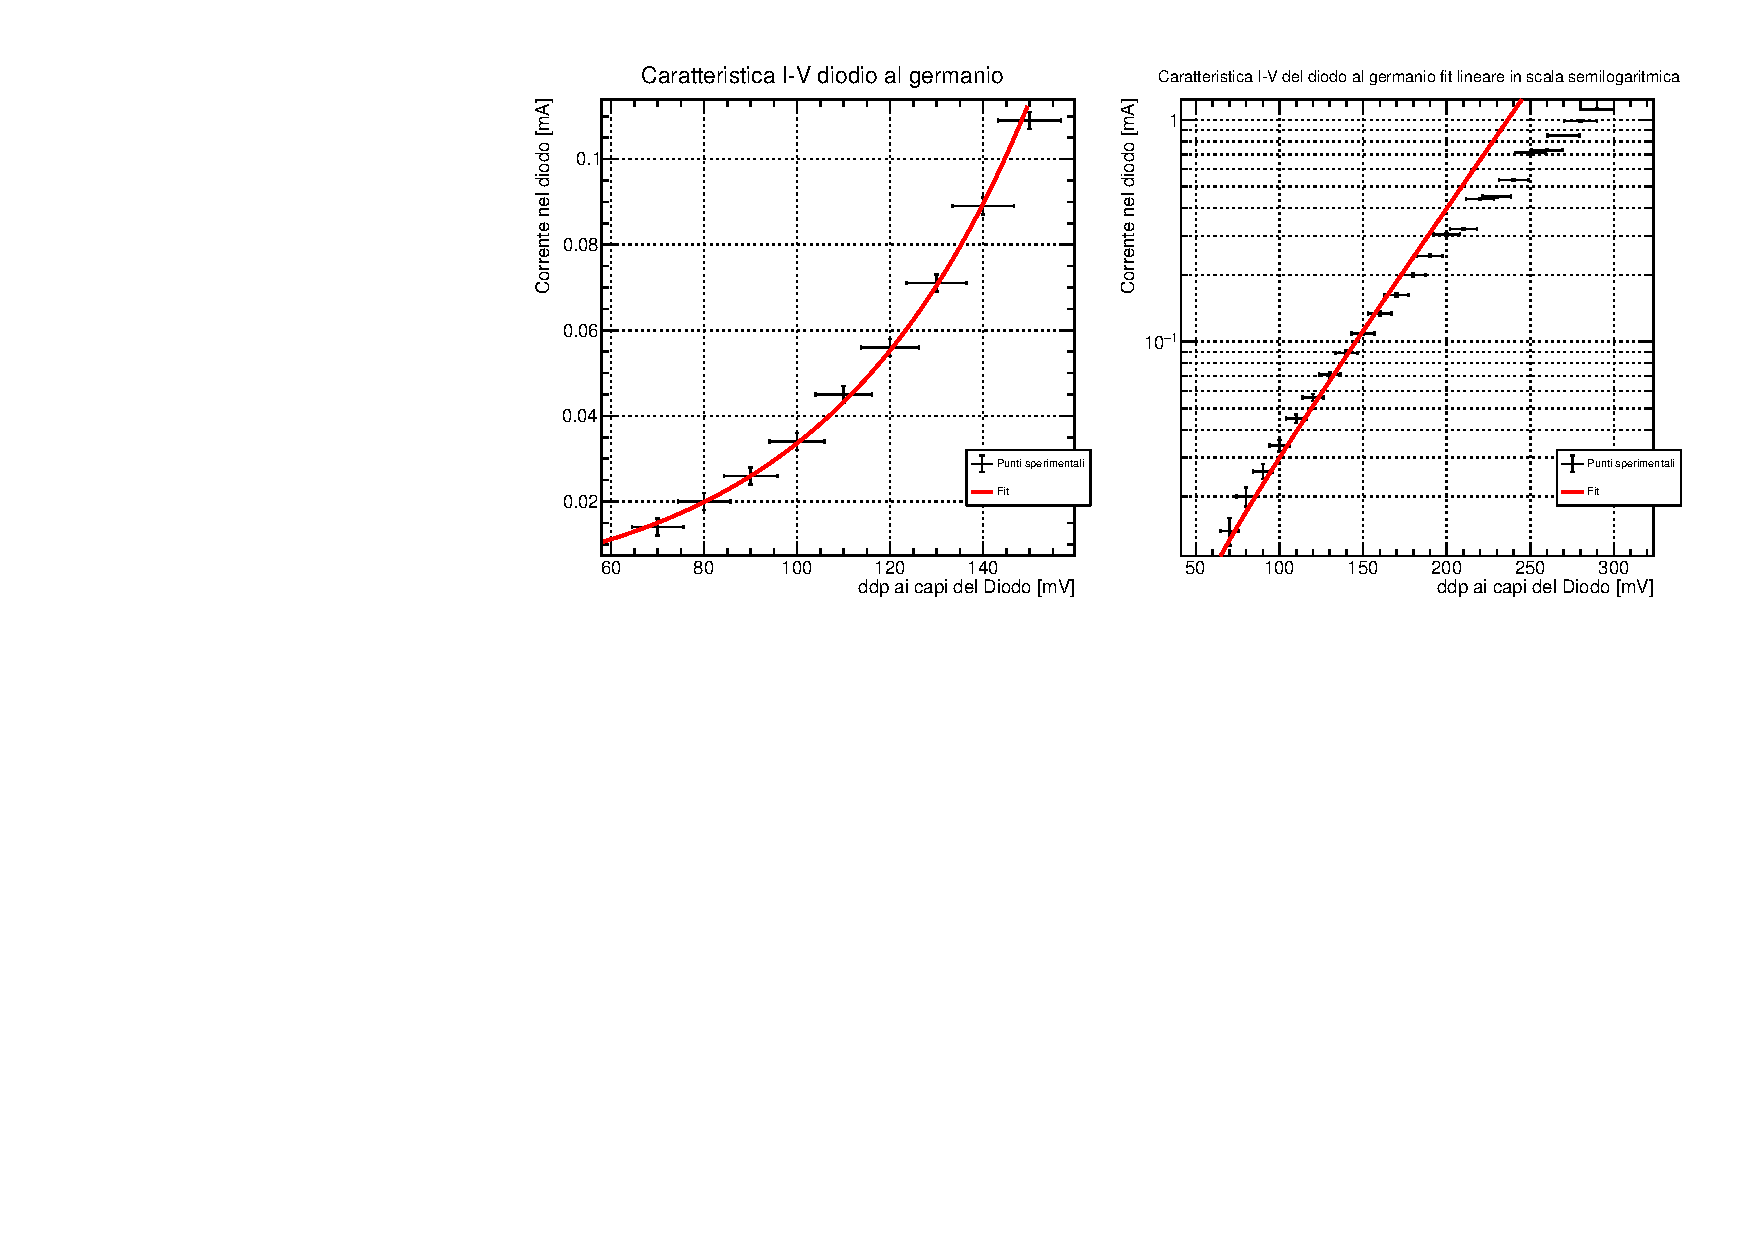
\includegraphics[width=0.8\linewidth]{../Germanio/canvas}
	\caption{Caratteristica I-V del diodo al Germanio: a sinistra sono riportati i punti nel range utilizzato per effettuare il fit esponenziale mentre a destra sono riportati tutti i punti sperimentali in scala semilogaritmica con fit lineare}
	\label{fig:germanio}
\end{figure}
Anche in questo caso osserviamo che le misure ottenute dai due fit sono compatibili tra loro seppur il fit lineare si riveli più preciso riuscendo a stimare con un errore minore il parametro $I_0$.
Notiamo però che il parametro misurato $\eta V_T$ non risulta in accordo con quello atteso; questo è dovuto a vari fattori tra cui l'impossibilità di misurare la temperatura di operazione della giunzione che varia il valore di questo parametro.
\section*{Conclusioni}
Le misure della caratteristica I-V dei due diodi si sono rivelate qualitativamente in accordo con la teoria riproducendo la legge del diodo ideale e manifestando anche una minor aderenza con questa a tensioni più alte, come è previsto dalla caratteristica di un diodo reale. 

Per il diodo al Silicio abbiamo ottenuto due misure di ogni parametro caratteristico, $I_0=(5\pm5)nA$ e $\eta V_T=(51\pm5)mV$ con fit esponenziale, e $I_0=(7.2\pm0.7)nA$ e $\eta V_T=(53\pm4)mV$ con fit lineare, in accordo tra di loro ed entrambe in accordo con i valori attesi. Per quanto riguarda il diodo al Germanio il fit esponenziale ha restituito $I_0=(4\pm1)\mu A$ e $\eta V_T=(43\pm5)mV$, in accordo con le stime del fit lineare $I_0=(2.6\pm0.3)\mu A$ e $\eta V_T=(40\pm3)mV$, ma entrambi in disaccordo con i valori attesi. Questa discrepanza è dovuta alle variazioni di temperatura della giunzione che fanno variare il valore di $\eta V_T$, combinate con gli errori strumentali.
\end{document}
